\chapter[Proposta]{Proposta}

Como já dito, a proposta deste trabalho é a construção de um \textit{framework} de definição de trajetória para robôs móveis, mais especificamente, algoritmos globais de definição de trajetória. Um mapa do ambiente é recebido da camada acima e o algoritmo cria um grafo a partir dele, definindo os caminhos livres que podem ser percorridos. Após isso é rodado um algoritmo de menor caminho (como Djikstra) para definir o caminho a ser percorrido pelo robô. 

A imagem abaixo demonstra as tarefas principais do \textit{framework}, bem como suas entradas e saídas. Essas entradas e saídas definem como ele se comunicará com as demais camadas do robô e as dependências dele para cumprir seu funcionamento. Cada tarefa apresentada se tornará um módulo do \textit{framework} e as interações entre eles as estruturas de dados utilizadas para se comunicarem.
 
\begin{figure}[h]
	\centering
	\label{fig18}
		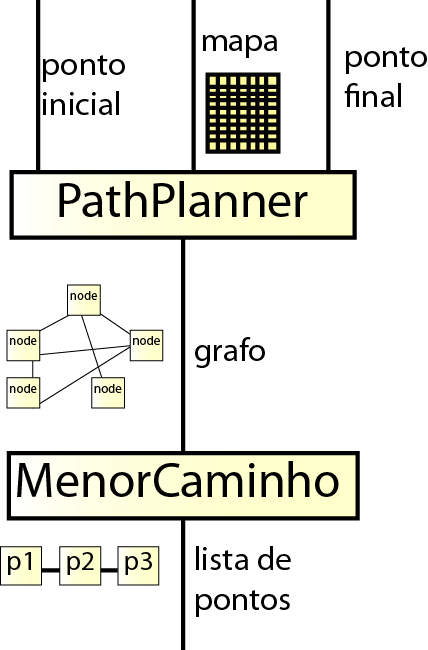
\includegraphics[keepaspectratio=true,scale=1]{figuras/framework.png}
	\caption{estrutura do funcionamento do \textit{framework}}
\end{figure} 

A arquitetura geral do robô será considerada como na imagem abaixo apresentada por Nehmzow (2003). Todas as abordagens da arquitetura de navegação seguiam uma lógica semelhante e apresentavam pequenas diferenças entre si. Assim sendo, esta estrutura mantêm as características apresentadas no capítulo anterior.

\begin{figure}[h]
	\centering
	\label{fig19}
		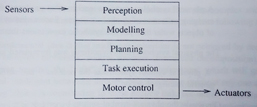
\includegraphics[keepaspectratio=true,scale=1]{figuras/arqusada.jpg}
	\caption{arquitetura a navegação considerada, Nehmzow (2003, pg 15)}
\end{figure}

Como a camada acima é responsável pelo mapeamento e entrega o mapa completo, os algoritmos globais e este \textit{framework} não precisam se preocupar com comunicação com os sensores. A camada abaixo recebe a lista de coordenadas para onde deve ir e cuida do controle dos motores para chegar neles considerando os graus de liberdade do robô (que varia de acordo com sua estrutura física). Assim, a camada a ser criada não se comunica nem com os sensores nem com os motores, o que lhe dá maior independência das configurações de robô. Com isso é esperado que o \textit{framework} funcione em variados tipos de robôs, não apenas nos \textit{differential steering} testados.

A seguir é definido como funcionará os detalhes do \textit{framework} levantados no capítulo anterior.

\section{O mapa}

Todo o processo se inicia com o recebimento dele para então operar sobre o mesmo. Dentre os tipos de mapa apresentados no capítulo anterior o mapa esperado pelo \textit{framework} será uma malha de ocupação. Junto com a matriz será recebido os valores para terreno ocupado e livre. A seguir deve ser marcado no mapa quais são os pontos iniciais e finais.

O \textit{framework} usa uma estrutura própria para armazenar estes dados, porém guarda referência aos dados originais da camada de sensoriamento, evitando o gasto excessivo de memória para a mesma informação. As alterações nos dados do mapa deverão ser revertidas ao fim do processamento do \textit{framework}, devolvendo ao mapa seus dados originais.

\section{A arquitetura}

A arquitetura de navegação costuma ser em camadas, como mostrado no capítulo anterior. Este \textit{framework} trabalhará dentro de uma destas camadas apenas e terá uma estrutura baseada em componentes. Uma arquitetura em camadas dentro de outra poderia gerar indireções desnecessárias, além de uma abordagem por componentes suprir melhor as necessidades do \textit{framework}.

Cada funcionalidade será um componente diferente, projetado para consumir o mínimo de memória e depender o mínimo de outros componentes e de bibliotecas externas (incluindo as próprias do Java). Cada módulo terá a preocupação de ser o mais auto-suficiente possível, tendo apenas as interações necessárias para o seu funcionamento. Cada um dos módulos será constantemente avaliado quando a seu acoplamento, coesão,  simplicidade e facilidade de compreensão. Estas características serão melhor definidas na seção 4.5.

diagramas, caixa-branca, topdown

\section{Componentes do framework}

explicar o componente e os padrões usados em cada um

\subsection{Map}
\subsection{Path Planner}
\subsection{Graph}
\subsection{Shortest Path}
\subsection{Controller}

\section{Hot-spots do framework}

\section{Boas práticas de programação}
citar também coesão, acoplamento, complexidade ciclomatica.